\chapter{Cinemática relativística}\label{ch:b3:relativistic-kinematics}

Os raios cósmicos que atingem a alta atmosfera criam múons a quinze
quilômetros de altura --- partículas instáveis que vivem, em média,
dois microssegundos. Dois microssegundos a quase a velocidade da luz
são seiscentos metros; e, no entanto, os detectores de múons ao nível
do mar disparam sem parar, contando partículas que percorreram vinte
vezes o alcance que lhes cabia. A solução desse paradoxo não é um
detalhe da física de partículas, mas uma revisão dos conceitos que
sustentam toda a física: o tempo transcorre de modo diferente para o
múon em movimento e para nós, e as distâncias encolhem ao longo do seu
movimento. Este capítulo constrói essa revisão --- a relatividade
restrita (Einstein, 1905) --- a partir de seus dois postulados: as
leis da física são as mesmas em todo \omterm{thm:b3:relativistic-kinematics:postulates}{referencial inercial}, e a luz no
vácuo tem a mesma velocidade em todos eles. Todo o resto decorre de
uma cinemática honesta: o enlace do espaço com o tempo na \omterm{thm:b3:relativistic-kinematics:lorentz}{transformação
de Lorentz}, a \omterm{prop:b3:relativistic-kinematics:dilation}{dilatação do tempo}, a \omterm{prop:b3:relativistic-kinematics:contraction}{contração dos comprimentos}, a nova
regra de \omterm{prop:b3:relativistic-kinematics:addition}{composição de velocidades} e a geometria --- o espaço-tempo e
seu intervalo invariante --- em que tudo isso se torna tão natural
quanto as rotações.

\section{Dois postulados contra o tempo absoluto}

\begin{remark}[De onde vem o conflito]\label{rem:b3:relativistic-kinematics:conflict}
A mecânica sempre teve um princípio de relatividade: dentro de um navio
que navega suavemente, nenhum experimento com bolas e pêndulos
denuncia o movimento (Galileu), e as leis de Newton valem em todo
\emph{\omterm{thm:b3:relativistic-kinematics:postulates}{referencial inercial}}, isto é, nos referenciais em movimento
retilíneo uniforme uns em relação aos outros. Mas o eletromagnetismo do
volume do segundo ano deduz uma velocidade definida para a luz,
$c = 1/\sqrt{\varepsilon_0\mu_0} =
\qty{3.00e8}{m/s}$, a partir de constantes da natureza, sem qualquer
menção a quem a mede --- e os experimentos concordam: a velocidade da
luz das estrelas que chega à Terra em movimento, medida ao longo das
estações, nunca varia (Michelson e Morley, 1887, e todos os seus
sucessores). A cinemática galileana, em que as velocidades se somam,
não consegue digerir uma velocidade que é a mesma para todos. Algo tem
de ceder, e é a nossa suposição de que o tempo e a \omterm{def:b3:relativistic-kinematics:event}{simultaneidade} são
absolutos.
\end{remark}

\begin{theorem}[Os postulados da relatividade restrita]\label{thm:b3:relativistic-kinematics:postulates}
\index{relatividade!postulados}\index{referencial inercial}
\emph{(i) Relatividade:} as leis da física tomam a mesma forma em todo
\omterm{thm:b3:relativistic-kinematics:postulates}{referencial inercial}; nenhum experimento distingue o repouso do
movimento uniforme. \emph{(ii) Luz:} a luz no vácuo se propaga com a
mesma velocidade $c$ em todo \omterm{thm:b3:relativistic-kinematics:postulates}{referencial inercial}, qualquer que seja o
movimento da fonte ou do observador.
\end{theorem}
\admitted

\begin{definition}[Eventos e simultaneidade]\label{def:b3:relativistic-kinematics:event}
\index{evento}\index{simultaneidade}
Um \emph{evento} é uma ocorrência pontual: um lugar definido \emph{e}
um instante definido --- uma faísca, um disparo de detector, um
decaimento. Cada \omterm{thm:b3:relativistic-kinematics:postulates}{referencial inercial} atribui a um evento suas
coordenadas $(t, x, y, z)$, usando réguas em repouso no referencial e
relógios sincronizados distribuídos por ele. Dois eventos são
\emph{simultâneos num referencial} quando os relógios desse referencial
lhes atribuem o mesmo $t$ --- e a primeira vítima dos postulados é que
essa noção depende do referencial.
\end{definition}

\begin{example}[O trem e os dois raios]\label{ex:b3:relativistic-kinematics:train}
Dois raios atingem as duas extremidades de um trem veloz, deixando
marcas no trem e nos trilhos. Para a observadora no solo, a meio
caminho entre as marcas, os dois clarões chegam juntos: as descargas
foram simultâneas para ela. O passageiro sentado no meio do trem,
porém, move-se na direção de um clarão e afastando-se do outro;
viajando a $c$ também no referencial dele, o clarão da frente o alcança
primeiro --- e, como ele está a igual distância das duas marcas
\emph{no trem}, deve concluir que a descarga da frente ocorreu
\emph{antes}. Nenhum dos dois está errado: a \omterm{def:b3:relativistic-kinematics:event}{simultaneidade} de \omterm{def:b3:relativistic-kinematics:event}{eventos}
separados não é um fato sobre o mundo, mas sobre o referencial. Todo
``paradoxo'' relativístico se dissolve aqui.
\end{example}

\begin{omfigure}
\begin{tikzpicture}[font=\small, >=Stealth]
  % ground view
  \begin{scope}
    \draw[thick] (-0.3,0) -- (10.3,0);
    \fill[omDef!18, draw=omDef, thick, rounded corners=2pt] (1.4,0.15) rectangle (8.6,1.05);
    \foreach \x in {2.2,3.4,4.6,5.8,7.0} \draw[omDef] (\x,0.35) rectangle (\x+0.7,0.85);
    \draw[->, very thick] (8.9,0.6) -- (9.9,0.6) node[right] {$v$};
    \node[omExo] at (1.4,1.75) {\Large$\downarrow$};
    \node[omExo] at (8.6,1.75) {\Large$\downarrow$};
    \node[omExo, font=\footnotesize] at (1.4,2.15) {raio A};
    \node[omExo, font=\footnotesize] at (8.6,2.15) {raio B};
    \fill (5,-0.02) circle (2pt);
    \node[font=\footnotesize] at (5,-0.4) {observadora no solo, no meio};
    \fill[omThm] (5,1.22) circle (2pt);
    \node[omThm, font=\footnotesize] at (5.1,1.55) {passageiro, meio do trem};
  \end{scope}
\end{tikzpicture}

{\small Dois raios marcam ao mesmo tempo o trem e os trilhos. A
observadora no solo, a meio caminho entre as marcas, recebe os clarões
juntos: simultâneos para ela. O passageiro corre ao encontro do clarão
B; ele o alcança primeiro e --- estando a igual distância das marcas em
seu próprio referencial --- ele conclui que B veio antes. A
\omterm{def:b3:relativistic-kinematics:event}{simultaneidade} é relativa.}
\end{omfigure}

\section{A transformação de Lorentz}

\begin{theorem}[Transformação de Lorentz]\label{thm:b3:relativistic-kinematics:lorentz}
\index{transformação de Lorentz}\index{fator gama@fator $\gamma$}
Seja o referencial $\mathcal R'$ em movimento com velocidade $v$ ao
longo do eixo $x$ do referencial $\mathcal R$, com as origens
coincidindo em $t = t' = 0$. Um \omterm{def:b3:relativistic-kinematics:event}{evento} $(t, x)$ de $\mathcal R$ tem em
$\mathcal R'$ as coordenadas
\[
x' = \gamma\,(x - vt) , \qquad
t' = \gamma\Big(t - \frac{v\,x}{c^2}\Big) , \qquad
\gamma = \frac{1}{\sqrt{1 - v^2/c^2}} ,
\]
com $y' = y$, $z' = z$; a transformação inversa é a mesma com
$v \to -v$. Para $v \ll c$, $\gamma \to 1$ e recupera-se o
$x' = x - vt$, $t' = t$ de Galileu. O fator $\gamma \ge 1$ --- apenas
$1$ nas velocidades cotidianas, $1.15$ a $c/2$, $7.1$ a $0.99c$ ---
mede todos os efeitos relativísticos deste capítulo.
\end{theorem}

\begin{proof}[Demonstração parcial]
A homogeneidade do espaço e do tempo obriga a transformação a ser
linear; a simetria entre os referenciais e o postulado da relatividade
a reduzem a $x' = \gamma(x - vt)$, $x = \gamma(x' + vt')$ com uma única
função incógnita $\gamma(v)$. Acompanhe um clarão de luz emitido na
origem comum: o postulado (ii) exige $x = ct$ \emph{e} $x' = ct'$.
Substituindo, $ct' = \gamma t(c - v)$ e $ct = \gamma t'(c + v)$;
multiplicando as duas equações, $c^2 = \gamma^2(c^2 - v^2)$, que é o
$\gamma$ enunciado. Eliminando $x'$ entre as duas relações lineares
obtém-se a fórmula do tempo. (A passagem de ``a luz concorda'' a ``a
transformação está completamente fixada'' --- sem qualquer alongamento
residual das direções transversais nem reescalonamento --- usa os
argumentos de simetria detalhados no
\cref{exo:b3:relativistic-kinematics:11}.)
\end{proof}

\begin{proposition}[Dilatação do tempo]\label{prop:b3:relativistic-kinematics:dilation}
\index{dilatação do tempo}\index{tempo próprio}
Um relógio em repouso em $\mathcal R'$ --- que bate com $x'$ fixo --- é
visto de $\mathcal R$ andar devagar: entre dois de seus tiques
separados pelo \emph{\omterm{prop:b3:relativistic-kinematics:dilation}{tempo próprio}} $\Delta\tau$ (o tempo do
referencial em que o relógio repousa), o referencial $\mathcal R$ mede
\[
\Delta t = \gamma\,\Delta\tau \ge \Delta\tau .
\]
Os relógios em movimento andam devagar --- todos eles, biológicos,
atômicos ou subatômicos, porque o que se dilata é o tempo em si, e não
um mecanismo.
\end{proposition}

\begin{proof}
Dois tiques no mesmo $x'$: a transformação inversa dá $\Delta t
= \gamma(\Delta t' + v\,\Delta x'/c^2) = \gamma\,\Delta\tau$, pois
$\Delta x' = 0$. A imagem do relógio de luz
(\cref{exo:b3:relativistic-kinematics:2}) dá o mesmo $\gamma$ só com
Pitágoras.
\end{proof}

\begin{proposition}[Contração dos comprimentos]\label{prop:b3:relativistic-kinematics:contraction}
\index{contração dos comprimentos}\index{comprimento próprio}
Uma haste de \emph{\omterm{prop:b3:relativistic-kinematics:contraction}{comprimento próprio}} $L_0$ (seu comprimento no
referencial em que repousa), em movimento longitudinal com velocidade
$v$, mede no laboratório
\[
L = \frac{L_0}{\gamma} \le L_0 .
\]
As dimensões transversais não mudam. Medir uma haste em movimento
significa localizar suas duas extremidades \emph{no mesmo instante do
laboratório} --- e, como a \omterm{def:b3:relativistic-kinematics:event}{simultaneidade} depende do referencial, o
comprimento também depende.
\end{proposition}

\begin{proof}
Marque as duas extremidades no mesmo tempo $t$ do laboratório: a
transformação dá $\Delta x' = \gamma(\Delta x - v\Delta t) = \gamma\,\Delta x$
com $\Delta t = 0$, e $\Delta x' = L_0$: logo $\Delta x = L_0/\gamma$.
\end{proof}

\begin{omfigure}
\begin{tikzpicture}[font=\small, >=Stealth]
  % light clock at rest
  \begin{scope}
    \draw[thick] (-0.7,0) -- (0.7,0);
    \draw[thick] (-0.7,2.2) -- (0.7,2.2);
    \draw[->, omExo, thick] (0,0.08) -- (0,2.12);
    \node[anchor=west] at (0.12,1.1) {$c\,\Delta\tau$};
    \node at (0,-0.55) {relógio em repouso: um tique};
  \end{scope}
  % moving light clock
  \begin{scope}[xshift=5.6cm]
    \draw[thick] (-0.7,0) -- (4.7,0);
    \draw[thick] (-0.7,2.2) -- (4.7,2.2);
    \draw[gray, dashed] (0,0) -- (0,2.2);
    \draw[gray, dashed] (4,0) -- (4,2.2);
    \draw[->, omExo, thick] (0,0.08) -- (1.96,2.12);
    \draw[->, omExo, thick] (2.04,2.12) -- (4,0.14);
    \node[rotate=47, anchor=south] at (0.85,1.0) {$c\,\Delta t/2$};
    \draw[->, thick] (0,-0.35) -- (4,-0.35);
    \node at (2,-0.75) {o espelho avança de $v\,\Delta t$};
    \node at (2,3.0) {$\Big(\dfrac{c\Delta t}{2}\Big)^2 = \Big(\dfrac{v\Delta t}{2}\Big)^2 + \Big(\dfrac{c\Delta\tau}{2}\Big)^2$};
  \end{scope}
\end{tikzpicture}

{\small O relógio de luz: um fóton que ricocheteia entre dois espelhos.
Visto do referencial em que o relógio se move, o fóton percorre um
caminho mais longo e inclinado à mesma velocidade $c$: o tique demora
mais, $\Delta t = \gamma\,\Delta\tau$, só por Pitágoras.}
\end{omfigure}

\begin{example}[O múon, explicado duas vezes]\label{ex:b3:relativistic-kinematics:muon}
Um múon a $v = 0.995c$ tem $\gamma = 10$. No nosso referencial, seu
relógio interno anda dez vezes mais devagar: seus dois microssegundos
de vida própria se esticam para vinte, e ele percorre seis quilômetros
em vez de seiscentos metros. No referencial do múon, sua vida são os
comuns \qty{2.2}{\micro s} --- mas a montanha que se precipita sobre
ele está contraída dez vezes, e cabe no percurso. Os dois referenciais
concordam sobre o único fato físico, \emph{se o múon chega ou não ao
detector}: a relatividade reembaralha tempos e comprimentos, jamais
desfechos (\cref{pb:b3:relativistic-kinematics:1}).
\end{example}

\begin{method}[Como não confundir os efeitos]\label{met:b3:relativistic-kinematics:method}
(1) Identifique os \emph{\omterm{def:b3:relativistic-kinematics:event}{eventos}} (emissão, chegada, tique,
decaimento), e não ``objetos''. (2) O \omterm{prop:b3:relativistic-kinematics:dilation}{tempo próprio} $\Delta\tau$
pertence ao único relógio presente nos dois \omterm{def:b3:relativistic-kinematics:event}{eventos}: todo outro
referencial mede mais, $\gamma\Delta\tau$. (3) O \omterm{prop:b3:relativistic-kinematics:contraction}{comprimento próprio}
$L_0$ pertence ao referencial em que a haste repousa: todo outro
referencial mede menos, $L_0/\gamma$. (4) Quando um ``paradoxo''
aparecer, procure os dois \omterm{def:b3:relativistic-kinematics:event}{eventos} espacialmente separados que estão
sendo silenciosamente chamados de simultâneos e pergunte: em qual
referencial? (5) Verifique o limite $v/c \to 0$ e lembre que
$\gamma - 1 \approx \tfrac12 v^2/c^2$ a baixas velocidades --- o
tamanho das correções relativísticas do dia a dia.
\end{method}

\section{Composição de velocidades; efeito Doppler}

\begin{proposition}[Composição relativística de velocidades]\label{prop:b3:relativistic-kinematics:addition}
\index{composição de velocidades}
Se um corpo se move com velocidade $u'$ ao longo de $x'$ no referencial
$\mathcal R'$, ele próprio em movimento com velocidade $v$ em relação a
$\mathcal R$, então $\mathcal R$ não mede $u' + v$, mas
\[
u = \frac{u' + v}{1 + u'v/c^2} .
\]
Para as velocidades cotidianas o denominador vale $1$ e Galileu
retorna; para $u' = c$ a fórmula dá $u = c$ qualquer que seja $v$ --- a
luz está a $c$ para todos, como foi construído; e nenhuma \omterm{prop:b3:relativistic-kinematics:addition}{composição de
velocidades} abaixo de $c$ jamais alcança $c$.
\end{proposition}

\begin{proof}
$u = \dd x/\dd t$ com a transformação inversa: $\dd x =
\gamma(\dd x' + v\,\dd t')$, $\dd t = \gamma(\dd t' + v\,\dd x'/c^2)$;
divida.
\end{proof}

\begin{example}[O coeficiente de Fresnel explicado]\label{ex:b3:relativistic-kinematics:fizeau}
A luz na água parada viaja a $c/n$. Na água que escoa com velocidade
$v$, Fizeau mediu (1851) o intrigante $c/n + v(1 - 1/n^2)$: não o
arrasto completo $c/n + v$. Componha $u' = c/n$ com $v$:
\[
u = \frac{c/n + v}{1 + v/nc}
\approx \Big(\frac{c}{n} + v\Big)\Big(1 - \frac{v}{nc}\Big)
\approx \frac{c}{n} + v\Big(1 - \frac{1}{n^2}\Big) ,
\]
até primeira ordem em $v/c$. Um resultado de bancada do século XIX,
então inexplicável, é a lei de \omterm{prop:b3:relativistic-kinematics:addition}{composição de velocidades} lida em
primeira ordem --- uma das confirmações discretas que Einstein citou em
1905.
\end{example}

\begin{proposition}[Efeito Doppler longitudinal]\label{prop:b3:relativistic-kinematics:doppler}
\index{efeito Doppler!relativístico}
Uma fonte de frequência própria $f_0$ que se afasta com velocidade
$v = \beta c$ ao longo da linha de visada é recebida em
\[
f = f_0\,\sqrt{\frac{1 - \beta}{1 + \beta}}
\qquad
\text{(aproximando-se: } \beta \to -\beta\text{)} .
\]
Dois efeitos se compõem: o alongamento clássico dos tempos de chegada,
porque cada crista parte de mais longe, e a lentidão relativística do
relógio da fonte --- o $\gamma$ que sobrevive mesmo a $90^\circ$ (o
efeito Doppler \emph{transversal}, pura \omterm{prop:b3:relativistic-kinematics:dilation}{dilatação do tempo}).
\end{proposition}

\begin{proof}
No referencial do receptor, a fonte emite cristas a cada
$\gamma/f_0$ (dilatação), cada uma partindo $v\gamma/f_0$ mais longe, de
modo que as cristas chegam a cada $\gamma(1 + \beta)/f_0 = \sqrt{(1+\beta)/
(1-\beta)}\,/f_0$.
\end{proof}

\begin{example}[O afastamento das galáxias]\label{ex:b3:relativistic-kinematics:redshift}
A linha do hidrogênio emitida em \qty{656.3}{nm} chega de uma galáxia
distante em \qty{689}{nm}: $f/f_0 = 0.953$, logo $\beta \approx 0.048$
--- a galáxia se afasta a \qty{14000}{km/s}. Aplicada por todo o céu,
essa única fórmula transformou espectros num mapa do universo em
expansão; o último capítulo deste livro retoma a história.
\end{example}

\section{O espaço-tempo e o intervalo invariante}

\begin{theorem}[O intervalo invariante]\label{thm:b3:relativistic-kinematics:interval}
\index{espaço-tempo}\index{intervalo}
Para dois \omterm{def:b3:relativistic-kinematics:event}{eventos} quaisquer, a combinação
\[
\Delta s^2 = c^2\,\Delta t^2 - \Delta x^2 - \Delta y^2 - \Delta z^2
\]
tem o mesmo valor em todo \omterm{thm:b3:relativistic-kinematics:postulates}{referencial inercial} --- a grandeza que a
relatividade conserva enquanto tempos e comprimentos se flexionam. Seu
sinal classifica o par: \emph{do tipo tempo} ($\Delta s^2 > 0$): algum
referencial leva os \omterm{def:b3:relativistic-kinematics:event}{eventos} ao mesmo lugar, e $\Delta s/c$ é o \omterm{prop:b3:relativistic-kinematics:dilation}{tempo
próprio} entre eles; \emph{do tipo espaço} ($\Delta s^2 < 0$): algum
referencial os torna simultâneos, e nenhum sinal pode conectá-los;
\emph{do tipo luz} ($\Delta s^2 = 0$): só a luz os conecta.
\end{theorem}

\begin{proof}
Substituição direta da \omterm{thm:b3:relativistic-kinematics:lorentz}{transformação de Lorentz}:
$c^2t'^2 - x'^2 = \gamma^2\big[(ct - \beta x)^2 - (x - \beta ct)^2
\big] = \gamma^2(1 - \beta^2)(c^2t^2 - x^2) = c^2t^2 - x^2$.
Quanto à classificação: levar os \omterm{def:b3:relativistic-kinematics:event}{eventos} ao mesmo lugar exige um
referencial de velocidade $v = \Delta x/\Delta t$, o que é possível
quando $|\Delta x| <
c\,|\Delta t|$ (tipo tempo); torná-los simultâneos exige $v =
c^2\Delta t/\Delta x$, o que é possível quando $|\Delta x| > c\,|\Delta t|$
(tipo espaço).
\end{proof}

\begin{remark}[A causalidade tem uma geometria]\label{rem:b3:relativistic-kinematics:causality}
\index{cone de luz}
Por cada \omterm{def:b3:relativistic-kinematics:event}{evento} passa o seu \emph{\omterm{rem:b3:relativistic-kinematics:causality}{cone de luz}}: os \omterm{def:b3:relativistic-kinematics:event}{eventos} que ele pode
influenciar (cone futuro), os que podem tê-lo influenciado (cone
passado) e o ``alhures'' do tipo espaço, causalmente isolado. Como um
par do tipo espaço tem ordem dependente do referencial --- alguns
referenciais veem A antes de B, outros B antes de A --- qualquer sinal
mais rápido que a luz permitiria a algum observador assistir a um
efeito precedendo sua causa. O limite de velocidade da relatividade não
diz respeito a motores; é o preço de uma história coerente.
\end{remark}

\begin{omfigure}
\begin{tikzpicture}[font=\small, >=Stealth, scale=0.92]
  % axes
  \draw[->] (-3.6,0) -- (3.9,0) node[right] {$x$};
  \draw[->] (0,-2.6) -- (0,3.4) node[above] {$ct$};
  % light cone
  \fill[omExo!14] (0,0) -- (2.9,2.9) -- (-2.9,2.9) -- cycle;
  \fill[omExo!14] (0,0) -- (2.4,-2.4) -- (-2.4,-2.4) -- cycle;
  \draw[omExo, thick] (-2.9,-2.9) -- (2.9,2.9);
  \draw[omExo, thick] (2.9,-2.9) -- (-2.9,2.9);
  \node[omExo, font=\footnotesize, anchor=west] at (2.6,2.35) {luz, $x = ct$};
  \node[font=\footnotesize] at (-0.55,2.35) {futuro};
  \node[font=\footnotesize] at (0,-2.1) {passado};
  \node[font=\footnotesize] at (3.05,0.7) {alhures};
  \node[font=\footnotesize] at (-3.0,0.7) {alhures};
  % worldline
  \draw[omDef, very thick] (-0.9,-2.5) .. controls (0.2,-0.6) and (-0.5,1.2) .. (0.75,3.1);
  \node[omDef, font=\footnotesize, anchor=west] at (0.85,3.25) {linha de universo};
  % event
  \fill (0,0) circle (2pt);
\end{tikzpicture}

{\small O espaço-tempo em torno de um \omterm{def:b3:relativistic-kinematics:event}{evento} (o ponto na origem). Seu
\omterm{rem:b3:relativistic-kinematics:causality}{cone de luz} separa o que ele pode afetar (futuro), o que pode tê-lo
afetado (passado) e o alhures do tipo espaço. As linhas de universo
materiais permanecem mais inclinadas que $45^\circ$ --- sempre dentro
do cone.}
\end{omfigure}

\begin{example}[A gêmea viajante]\label{ex:b3:relativistic-kinematics:twins}
Uma gêmea voa até uma estrela a $8$ anos-luz a $0.8c$
($\gamma = 5/3$) e volta. Tempo na Terra: $2 \times 8/0.8 =
\qty{20}{yr}$. O \omterm{prop:b3:relativistic-kinematics:dilation}{tempo próprio} da viajante: $20/\gamma = \qty{12}{yr}$
--- oito anos mais jovem, e sem paradoxo algum: as situações das gêmeas
\emph{não} são simétricas, pois uma linha de universo é reta (inercial
do início ao fim) e a outra tem um vinco na virada. Entre dois \omterm{def:b3:relativistic-kinematics:event}{eventos}
fixos, a linha de universo reta é a de \emph{maior} \omterm{prop:b3:relativistic-kinematics:dilation}{tempo próprio} ---
na geometria do espaço-tempo, o desvio vive menos. O efeito é medido
rotineiramente: relógios atômicos levados a dar a volta ao mundo
discordam de seus irmãos que ficaram em casa exatamente pelos
nanossegundos previstos (\cref{pb:b3:relativistic-kinematics:1}).
\end{example}

\begin{omfigure}
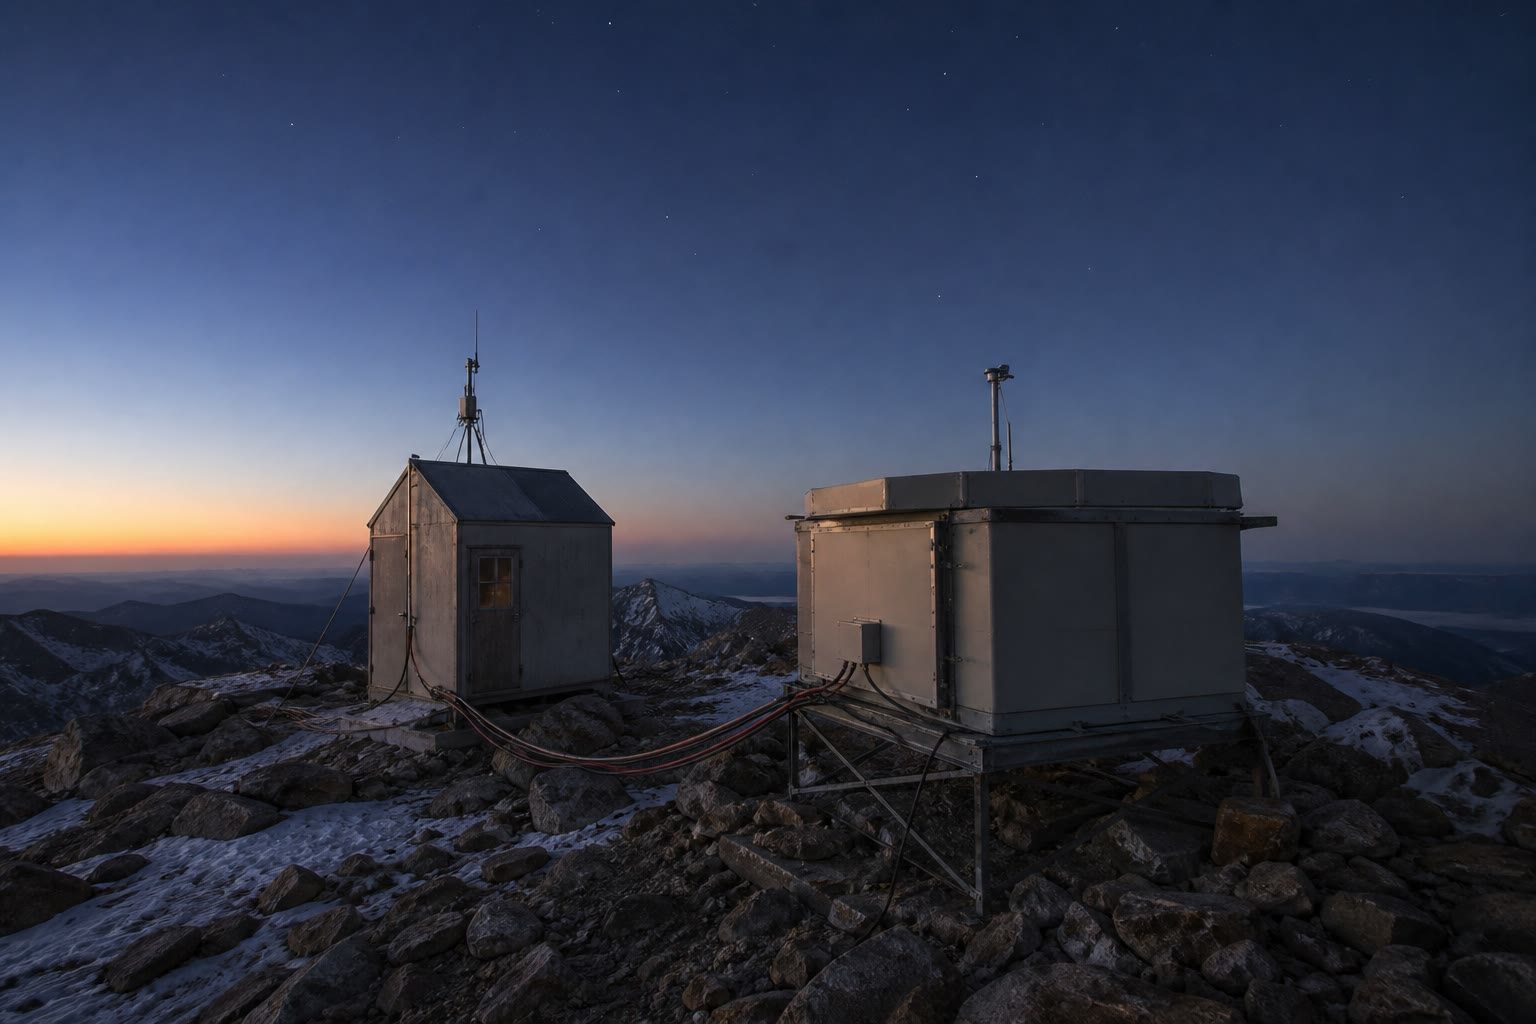
\includegraphics[width=0.58\linewidth]{images/book5/ai/b5-04-cosmic-ray-station.jpg}

{\small Uma estação de raios cósmicos em altitude. Os múons que ela conta, nascidos dez quilômetros acima, chegam até ela apenas porque os relógios em movimento andam devagar --- a \omterm{prop:b3:relativistic-kinematics:dilation}{dilatação do tempo}, medida todas as noites em cumes de montanha.}
\end{omfigure}

\section{Exercícios}

\begin{exercise}[$\star$]\label{exo:b3:relativistic-kinematics:1}
Calcule $\gamma$ para $v/c = 0.1$, $0.5$, $0.9$, $0.99$, $0.999$. Para
a Estação Espacial Internacional (\qty{7.7}{km/s}), calcule
$\gamma - 1$ pela aproximação de baixa velocidade e o tempo que sua
tripulação ``ganha'' (ou perde?) por missão de seis meses em relação a
um relógio no solo, ignorando a gravidade.
\end{exercise}

\begin{exercise}[$\star$]\label{exo:b3:relativistic-kinematics:2}
O relógio de luz da figura: (a) escreva o tique $\Delta\tau =
2d/c$ do relógio em repouso ($d$ é o espaçamento entre os espelhos);
(b) a partir de Pitágoras no referencial em que ele se move com
velocidade $v$, deduza $\Delta t =
\gamma\Delta\tau$; (c) por que o argumento exige que a distância
transversal $d$ seja a mesma nos dois referenciais? (d) Dê o argumento
(duas réguas idênticas passando uma pela outra) de que os comprimentos
transversais não podem mudar.
\end{exercise}

\begin{exercise}[$\star$]\label{exo:b3:relativistic-kinematics:3}
Um múon é criado a \qty{15}{km} de altitude com $v = 0.999c$. (a) Seu
$\gamma$ e sua vida média no nosso referencial. (b) A distância média
que percorre. (c) A espessura da atmosfera no referencial dele. (d) Que
fração desses múons chega ao solo, com e sem relatividade (lei de
decaimento $\eu^{-t/\tau}$, $\tau = \qty{2.2}{\micro s}$)?
\end{exercise}

\begin{exercise}[$\star$]\label{exo:b3:relativistic-kinematics:4}
Dois \omterm{def:b3:relativistic-kinematics:event}{eventos} sobre o eixo $x$: A em $(t = 0, x = 0)$, B em $(t =
\qty{2}{\micro s}, x = \qty{300}{m})$. (a) Calcule $\Delta s^2$: tipo
tempo ou tipo espaço? (b) A pode causar B? (c) Encontre a velocidade do
referencial em que A e B ocorrem no mesmo lugar, e o \omterm{prop:b3:relativistic-kinematics:dilation}{tempo próprio}
entre eles ali. (d) As mesmas três perguntas para B em
$(\qty{1}{\micro s}, \qty{600}{m})$ --- que referencial existe agora, e
qual não existe?
\end{exercise}

\begin{exercise}[$\star\star$]\label{exo:b3:relativistic-kinematics:5}
Os satélites do GPS orbitam a $v = \qty{3.87}{km/s}$. (a) Calcule $\gamma -
1$. (b) De quanto o relógio de um satélite atrasa em relação a um
relógio no solo por dia, só pela \omterm{prop:b3:relativistic-kinematics:dilation}{dilatação do tempo}? (c) O
posicionamento funciona cronometrando sinais que viajam a $c$: que erro
de posição corresponde a um dia de deriva relativística restrita não
corrigida? (d) A correção completa (com a gravidade, tratada no
espírito do último capítulo) é de $+38\,\unit{\micro s}$ por dia, com o
desvio gravitacional para o azul \emph{vencendo} a \omterm{prop:b3:relativistic-kinematics:dilation}{dilatação do tempo}:
o que o sinal lhe diz sobre qual efeito é maior a \qty{20200}{km} de
altitude?
\end{exercise}

\begin{exercise}[$\star\star$]\label{exo:b3:relativistic-kinematics:6}
(a) Uma nave a $0.8c$ lança uma sonda para a frente a $0.8c$ em relação
a si mesma: qual é a velocidade da sonda para nós? (b) Duas naves se
aproximam uma da outra, cada uma a $0.9c$ no nosso referencial: qual é
a velocidade relativa delas? (c) Mostre, a partir da lei de composição,
que $u' < c$ e $v < c$ implicam $u < c$ (fatore a expressão $c - u$).
(d) Um ponteiro laser varrido sobre a face da Lua pode pintar uma
mancha que se desloca mais rápido que $c$: por que isso não viola lei
alguma?
\end{exercise}

\begin{exercise}[$\star\star$]\label{exo:b3:relativistic-kinematics:7}
O dubleto do sódio em \qty{589.0}{nm} chega de uma estrela em
\qty{575.0}{nm}. (a) Ela se aproxima ou se afasta? Com que velocidade?
(b) Com que velocidade a luz visível (\qty{550}{nm}) seria deslocada
para o infravermelho próximo (\qty{1100}{nm})? (c) Para $\beta \ll 1$,
mostre que $\Delta\lambda/\lambda \approx \beta$ e dê a regra prática
em km/s por \unit{\angstrom} em \qty{600}{nm}. (d) Uma fonte que
circula a distância constante exibe um desvio mesmo sem movimento
radial: que efeito é esse, e de que ordem em $\beta$?
\end{exercise}

\begin{exercise}[$\star\star$]\label{exo:b3:relativistic-kinematics:8}
A vara e o celeiro. Uma vara de \qty{20}{m} é levada a $\gamma = 2$ em
direção a um celeiro de \qty{10}{m} com duas portas. (a) O comprimento
da vara no referencial do celeiro: ela cabe? (b) No referencial do
corredor, o \emph{celeiro} tem \qty{5}{m} de comprimento: como ambos
podem estar certos? Identifique os dois \omterm{def:b3:relativistic-kinematics:event}{eventos} (``a porta da frente
se fecha'', ``a porta de trás se abre'') e compare a ordem temporal
deles nos dois referenciais. (c) Calcule o tempo entre esses \omterm{def:b3:relativistic-kinematics:event}{eventos} em
cada referencial, supondo o fechamento simultâneo no celeiro. (d)
Enuncie a moral numa frase (que suposição silenciosa o ``paradoxo''
fez?).
\end{exercise}

\begin{exercise}[$\star\star$]\label{exo:b3:relativistic-kinematics:9}
Um foguete de \omterm{prop:b3:relativistic-kinematics:contraction}{comprimento próprio} \qty{100}{m} passa por uma estação
espacial a $0.6c$. (a) Quanto tempo marca o relógio da estação entre a
passagem do nariz e a da cauda? (b) A mesma pergunta para um relógio do
foguete que vê a estação (de \omterm{prop:b3:relativistic-kinematics:contraction}{comprimento próprio} \qty{300}{m}) passar.
(c) A estação dispara duas garras de acoplamento simultaneamente (no
referencial dela), a \qty{80}{m} de distância: qual é o tempo entre os
dois disparos para o foguete, e qual dispara primeiro? (d) Verifique
que $\Delta s^2$ coincide nos dois referenciais para o par de \omterm{def:b3:relativistic-kinematics:event}{eventos}
das garras.
\end{exercise}

\begin{exercise}[$\star\star\star$]\label{exo:b3:relativistic-kinematics:10}
As gêmeas, por inteiro. Estela voa a $0.8c$ até uma estrela a
\qty{8}{ly} de distância (no referencial da Terra) e volta a $0.8c$;
Terra fica. (a) Calcule o tempo decorrido para cada gêmea. (b) No
referencial de ida de Estela, a que distância está a estrela e quanto
tempo lhe toma a perna de ida? (c) Logo antes e logo depois da virada,
o que Estela calcula para ``a hora que é agora na Terra'' (use o termo
$vx/c^2$)? Mostre que sua contabilidade salta anos no vinco --- e que
esse salto é exatamente o que reconcilia os totais. (d) Explique por
que nenhum argumento simétrico pode ser feito do lado de Estela.
\end{exercise}

\begin{exercise}[$\star\star\star$]\label{exo:b3:relativistic-kinematics:11}
Deduzir Lorentz honestamente. (a) Argumente, a partir da
homogeneidade, que a transformação deve ser linear. (b) Supondo
$x' = \gamma(x - vt)$ e, pelo princípio da relatividade,
$x = \gamma(x' + vt')$, deduza $t'$ em função de $t$ e $x$ sem usar a
luz. (c) Mostre que exigir $x = ct \Rightarrow x' = ct'$ fixa $\gamma$
no valor enunciado. (d) Onde exatamente o argumento usou cada
postulado?
\end{exercise}

\begin{exercise}[$\star\star\star$]\label{exo:b3:relativistic-kinematics:12}
Rapidez. Defina $\varphi$ por $\tanh\varphi = \beta$. (a) Mostre que a
\omterm{thm:b3:relativistic-kinematics:lorentz}{transformação de Lorentz} se lê $ct' = ct\cosh\varphi - x\sinh\varphi$,
$x' = x\cosh\varphi - ct\sinh\varphi$: uma ``rotação'' por um ângulo
imaginário, que preserva $c^2t^2 - x^2$ como as rotações preservam
$x^2 + y^2$. (b) Mostre que compor velocidades \emph{soma as
rapidezes}: $\varphi =
\varphi_1 + \varphi_2$, e recupere a lei de composição a partir de
$\tanh(\varphi_1 + \varphi_2)$. (c) Um foguete acelera a $g$ no seu
próprio referencial: admitindo que sua rapidez cresce como
$\dd\varphi = g\,
\dd\tau/c$, encontre $\beta(\tau)$ e quanto \omterm{prop:b3:relativistic-kinematics:dilation}{tempo próprio} ele leva
para chegar a $0.99c$. (d) Por que a rapidez pode crescer para sempre,
enquanto $\beta$ não pode?
\end{exercise}

\begin{omfigure}
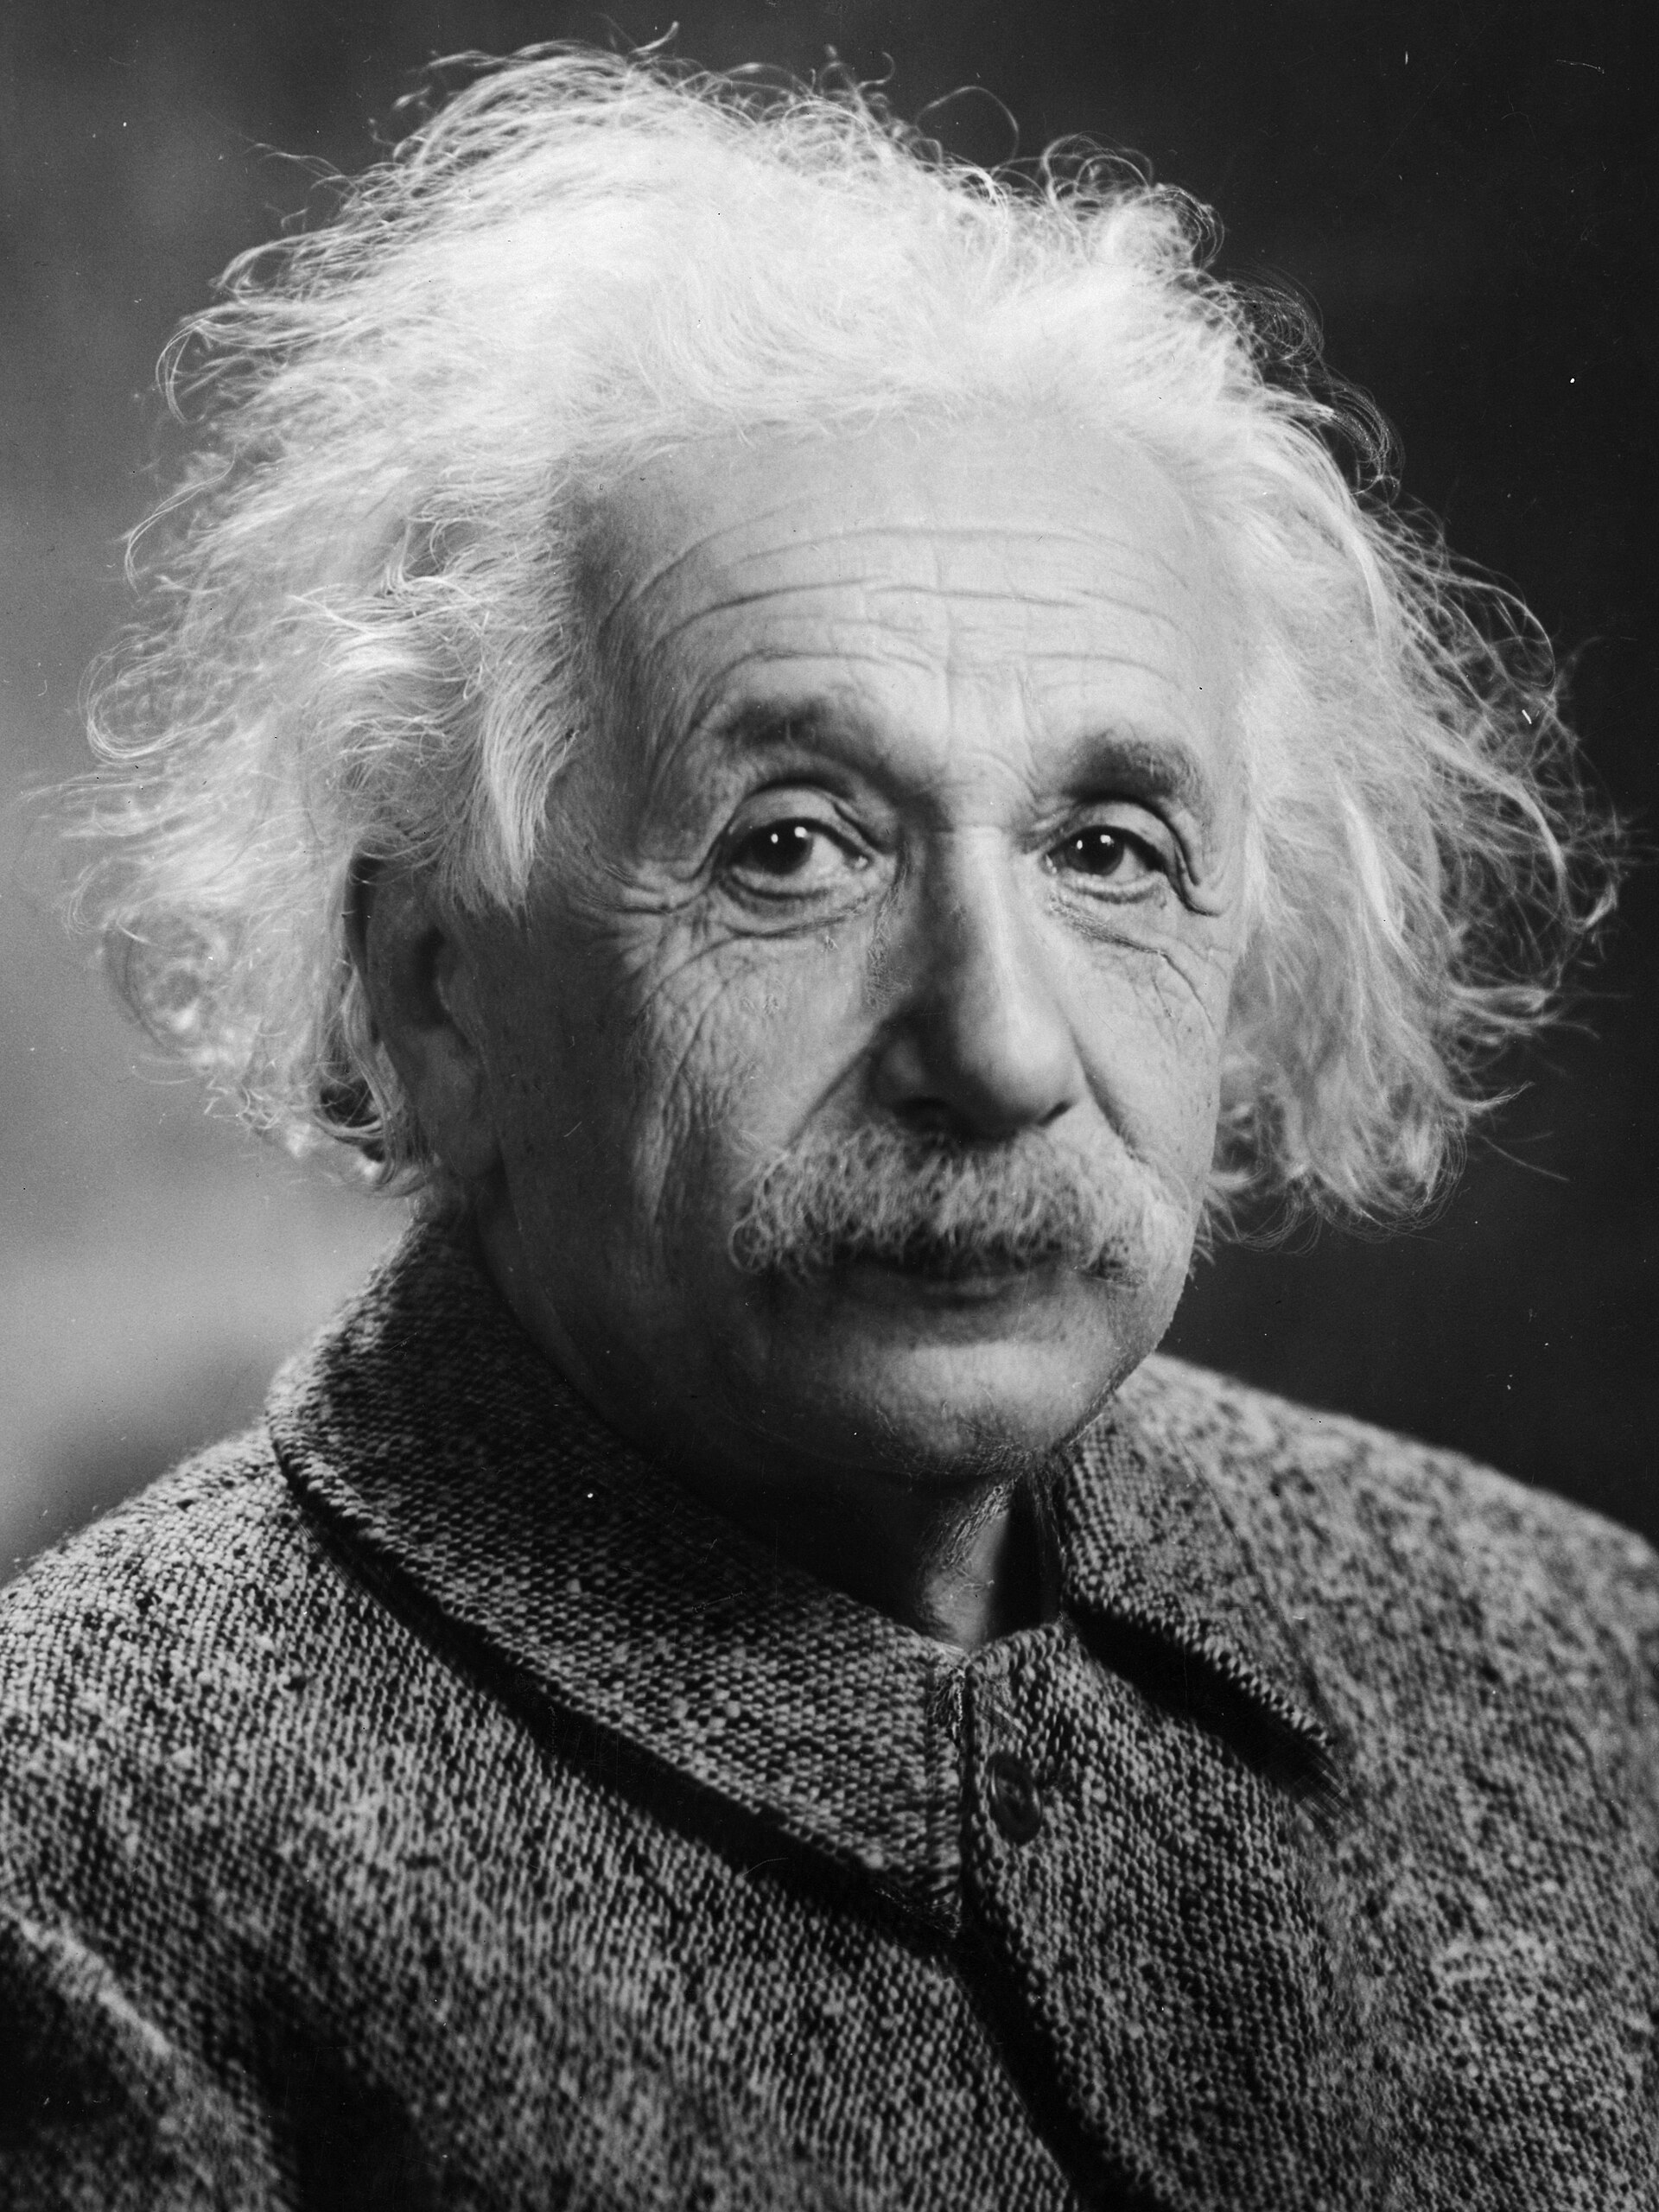
\includegraphics[width=0.34\linewidth]{images/book5/photo-einstein-1947.jpg}

{\small Albert Einstein (fotografia de Orren Jack Turner, 1947, domínio público). O artigo de 1905 sobre a relatividade reconstruiu a cinemática a partir de dois postulados --- este capítulo, essencialmente inalterado, é aquele artigo com exercícios.}
\end{omfigure}

\section{Problema: O experimento no céu}

\begin{problem}[{Problema de fim de semana --- múons, relógios de
montanha e a prova de que o tempo se dilata}]\label{pb:b3:relativistic-kinematics:1}
O teste inicial mais limpo da \omterm{prop:b3:relativistic-kinematics:dilation}{dilatação do tempo} não usou aparelho de
laboratório algum: a natureza fornece relógios relativísticos aos
milhares, que chovem sobre todas as montanhas. Este problema
reconstrói o experimento de Frisch e Smith (1963) e depois traz a mesma
física para os aviões de linha e os satélites de navegação. Dados: vida
média própria do múon $\tau =
\qty{2.20}{\micro s}$; o decaimento é exponencial, com uma fração
$\eu^{-t/\tau}$ dos múons sobrevivendo a um \omterm{prop:b3:relativistic-kinematics:dilation}{tempo próprio} $t$; $c =
\qty{3.00e8}{m/s}$; monte Washington: diferença de altitude $h =
\qty{1907}{m}$ entre os dois detectores.

\medskip\noindent\textbf{Parte I --- Relógios que chovem do céu.}
\begin{enumerate}
  \item Prótons cósmicos atingem núcleos no alto da atmosfera e os
        destroços decaem em múons por volta de \qty{15}{km} de
        altura. Por que uma população de partículas instáveis
        idênticas é um \emph{relógio}?
  \item Calcule $c\tau$, o alcance natural de uma vida média de múon.
  \item Sem relatividade, que fração dos múons nascidos a
        \qty{15}{km} e viajando essencialmente a $c$ chegaria ao
        solo? (Dê o expoente; o número em si é absurdo.)
  \item Os detectores ao nível do mar contam múons em abundância:
        enuncie a contradição numa frase.
  \item O fluxo ao nível do mar é de cerca de um múon por centímetro
        quadrado por minuto: estime quantos múons atravessam sua mão
        estendida a cada segundo, e seu corpo entre duas batidas do
        coração.
  \item O experimento selecionou múons de velocidade $0.995c$:
        calcule o $\gamma$ deles.
  \item Frisch e Smith contaram $563 \pm 10$ múons por hora no cume.
        Por que medir em duas altitudes do \emph{mesmo} chuveiro em
        vez de confiar na história da criação a \qty{15}{km}?
\end{enumerate}

\medskip\noindent\textbf{Parte II --- A medida na montanha.}
\begin{enumerate}[resume]
  \item Quanto tempo dura a viagem de \qty{1907}{m} a $0.995c$ no
        referencial da montanha?
  \item Sem \omterm{prop:b3:relativistic-kinematics:dilation}{dilatação do tempo}, que fração sobrevive a essa viagem, e
        quantos múons por hora deveriam chegar ao detector de baixo?
  \item Com a \omterm{prop:b3:relativistic-kinematics:dilation}{dilatação do tempo}, quanto tempo \emph{próprio}
        transcorre para o múon durante a viagem?
  \item Preveja a fração sobrevivente e a contagem por hora com a
        relatividade.
  \item A contagem medida embaixo foi de $408 \pm 9$ por hora. Compare
        as duas previsões com os dados e diga qual teoria sobrevive ao
        encontro com a montanha.
  \item A partir da razão medida $408/563$, extraia o fator de
        dilatação \emph{experimental} e compare-o com $\gamma = 10$.
        (Os múons desaceleram um pouco na blindagem rochosa, de modo
        que o $\gamma$ efetivo fica um pouco abaixo do valor do cume
        --- Frisch e Smith encontraram $8.8 \pm
        0.8$.)
\end{enumerate}

\medskip\noindent\textbf{Parte III --- A versão do próprio múon.}
\begin{enumerate}[resume]
  \item No referencial do múon, qual é a altura do monte Washington?
  \item Quanto tempo a montanha leva para desfilar por ele, e que
        fração dos múons decai nesse tempo? Verifique que coincide com
        a previsão da Parte II.
  \item Os dois referenciais discordam sobre o que se dilatou (o nosso
        tempo?\ a montanha dele?), mas concordam sobre a contagem: que
        tipo de grandeza é a contagem, e por que todos os referenciais
        devem concordar sobre ela?
  \item Calcule o intervalo $\Delta s^2$ entre a criação no cume e a
        chegada embaixo, no referencial da montanha, e verifique que
        $\Delta s/c$ é igual ao \omterm{prop:b3:relativistic-kinematics:dilation}{tempo próprio} do múon da Parte II.
  \item Um cético objeta: ``talvez seja a altitude, e não a
        velocidade, que muda as taxas de decaimento''. Que controle a
        dependência medida em $\gamma$ (múons mais lentos dilatam
        menos) oferece?
  \item Os anéis de armazenamento modernos mantêm múons a
        $\gamma = 29.3$ e medem vidas médias com precisão de
        $\num{e-3}$: o que eles encontram, e o que uma órbita circular
        acrescenta ao teste (qual das gêmeas é o múon)?
\end{enumerate}

\medskip\noindent\textbf{Parte IV --- De volta à Terra: aviões e
satélites.}
\begin{enumerate}[resume]
  \item Um avião de linha voa a \qty{250}{m/s} num voo de
        \qty{40}{h} ao redor do mundo. Usando
        $\gamma - 1 \approx v^2/2c^2$, calcule o atraso
        relativístico restrito do seu relógio, em nanossegundos.
  \item Os relógios de césio resolvem nanossegundos com facilidade; os
        voos de 1971 confirmaram a previsão (uma vez incluído o
        empurrão contrário da gravidade, maior em altitude). Por que os
        dois efeitos precisam ser separados voando \emph{tanto} para
        leste quanto para oeste?
  \item Um satélite do GPS ($v = \qty{3.87}{km/s}$) acumula que atraso
        de relógio relativístico restrito por dia, em microssegundos?
  \item Sem correção, quantos quilômetros de erro de distância
        \emph{uma semana} dessa deriva sozinha produziria?
  \item A correção completa do GPS, de $+38\,\unit{\micro s}$ por dia
        com a gravidade incluída, é embutida nos relógios dos
        satélites antes do lançamento: o que um navegador observaria
        em poucas horas se ela não existisse?
  \item Resuma o resultado central: uma montanha, dois contadores e
        relógios de $2.2\,\unit{\micro s}$ mediram a \omterm{prop:b3:relativistic-kinematics:dilation}{dilatação do
        tempo} em $\gamma \approx 9$ com $10\%$ de precisão em 1963 ---
        e a mesma física é corrigida, a cada segundo, em todo telefone
        que sabe onde está.
\end{enumerate}
\end{problem}
